\begin{frame}{Realism vs. Antirealism (and Bohr)}

\begin{center}
  \begin{tikzpicture}[every node/.style={align=center}]
    % Position realism box
    \node (realism) at (-3,0) [rectangle, draw, thick, minimum width=4cm, minimum height=1.5cm] 
      {Realism \\ \small Science aims at truth \\ about an objective reality};

    % Position antirealism box with xshift
    \node (antirealism) at (3,0) [rectangle, draw, thick, minimum width=4cm, minimum height=1.5cm] 
      {Antirealism \\ \small Science organizes experience; \\ truth may not apply};

    % Position Bohr oval below and centered
    \node (bohr) at (0,-2.7) [ellipse, draw=blue, very thick, minimum width=5.2cm, minimum height=1.6cm, fill=blue!10]
      {Bohr \\ \small ``Unambiguous communication'' \\ but not about ``things-in-themselves''};

    % Arrows
    \draw[<->, thick] (realism) -- (antirealism);
  \end{tikzpicture}
\end{center}

\vspace{0.5em}
\begin{itemize}
  \item Is Bohr a realist about classical concepts?
  \item Or an antirealist about quantum entities?
  \item He challenges the dichotomy itself.
\end{itemize}

\end{frame}



\begin{frame}{Favrholdt on Bohr}
  \begin{center}
    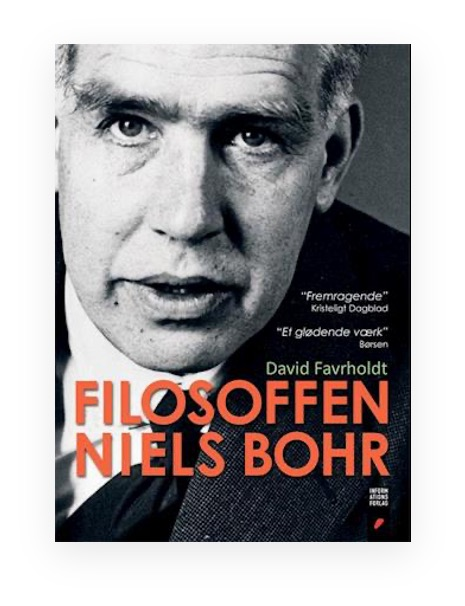
\includegraphics[width=0.45\linewidth]{favrholdt-filosoffen.jpg}%
    \hfill
    
\includegraphics[width=0.45\linewidth]{favrholdt-background.jpg}
  \end{center}
\end{frame}

\begin{frame}{Favrholdt on Bohr}
  
  ``Of course, a lot has already been written about Bohr's philosophy,
  but unfortunately not many people have been able to see the depth of
  it and its new vision when it comes to traditional philosophical
  issues.'' \citep{favrholdt2015} 

  ``I consider Niels Bohr to be one of the greatest thinkers in human
  history.'' \citep{favrholdt2015}

\nocite{favrholdt-background}  

\end{frame}

\begin{frame}{With friends like Max Jammer \dots }

``Misled by superficial coincidences, [Jammer] imagines that Bohr's
  thought has been influenced, through Høffding, by Kierkegaard and
  William James. There can be no doubt that his surmise is
  unfounded. Bohr was a completely independent thinker; from early
  youth, he developed his epistemological ideas single-handed.

  \bigskip \dots [Jammer] somehow went astray and ponderously built in
  a completely fictitious `Kierkegaard-Høffding' ideology into the
  discussion of Bohr's work.''

  \medskip (Rosenfeld, \emph{Nuclear Physics}, 1969)

\end{frame}



%%% Local Variables:
%%% mode: latex
%%% TeX-master: t
%%% End:
